\section{Where Is the Decision Made?}
\label{sec:measure}

Before training, we measure. All studies in this section use no training and run on real steps
sampled by the policy in the format above.

\subsection{GACA's step score is mostly path noise}
\label{sec:noise}
GACA's gate reads the mean NLL of the one response that was sampled. Exact token entropy,
$-\sum_v \pi(v)\log\pi(v)$ over the vocabulary, is available from the same forward pass and does not
depend on which token was drawn, so it removes the single-sample noise of the NLL at each position. On
7,864 step rows from the first five iterations of a GACA-family run, the two scores agree almost
perfectly (Pearson 0.94, within-trajectory Spearman 0.90): replacing NLL by exact entropy moves
$\lambda_t$ by more than 0.1 on only 0.9\% of steps. Averaging over $\sim$95 tokens already cancels
token-level sampling noise. The noise that remains is of another kind. At anchor states visited at
least twice in a group (575 states), visits to the \emph{same} state differ only in which reasoning
path was sampled, and that within-state variation accounts for 87\% of the variance of the NLL score
(85\% for exact entropy). GACA's criticality score is therefore mostly a property of the sampled path,
not of the state whose criticality it is meant to certify, which may explain why the paper's own
random-permutation control is needed to show that the gate's placement matters. Averaging across visits
(GACA-LOO) removes this noise but also the per-visit contrast; we test it in \cref{sec:results}.

\subsection{A counterfactual flip test}
To find where a decision is made inside a response, we intervene on it. For a step with response of
$L$ tokens and issued command $a^\star$, we cut the response after $j$ tokens at about 18 points
(every $L/16$ tokens plus the \texttt{<action>} tag), resample the remainder 8 times at temperature 1,
and record $F(j)$, the fraction of continuations whose command differs from $a^\star$. $F$ falls from
$F(0)$ (resample everything) to $F(L) = 0$, and its drop across a segment,
$F(c_k) - F(c_{k+1})$, is the share of the decision settled inside it. Because ALFWorld is
deterministic, an unchanged command implies an identical next state, so this is an exact step-level
relevance measure. We sample 320 valid steps from base-policy rollouts on 48 training games, which costs
44k continuations and about five minutes on one GPU with vLLM. The study is run twice on disjoint game
sets: once to design weighting schemes and once held out to test them.

Decisions are genuinely open and are made in the reasoning. Resampling a whole response changes the
command 72\% of the time, and 82\% of the decision mass is settled before the \texttt{<action>} tag.
\Cref{fig:deciles} shows where. Decision importance is spread through the reasoning and peaks in its
last tenth, where the model commits (18.8\%). Entropy follows a different profile: it is high in the
middle of the reasoning and lowest at the end (2.8\%), because once the model has committed, the tokens
that express the commitment look certain.

\begin{figure}[t]
\centering
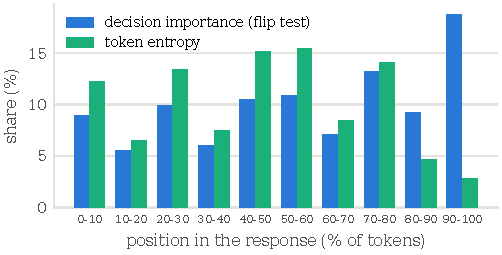
\includegraphics[width=\linewidth]{figs/deciles.pdf}
\caption{\textbf{Where the decision is made vs.\ where the entropy is}, by position in the response
(held-out flip test, 320 steps). The final tenth of a response holds 18.8\% of the decision but 2.8\%
of the token entropy.}
\label{fig:deciles}
\end{figure}

\subsection{Which signal locates the decision?}
We score each token-weighting scheme by the share of its credit that lands on decision importance,
$\sum_k m_k\, d_k$ for credit shares $m_k$ and importance shares $d_k$ over the fine flip-test segments,
relative to uniform credit (GACA), and by total-variation distance to importance. \Cref{fig:oracle}
summarizes. Token entropy, the signal behind single-turn ``forking token''
methods~\cite{wang2025beyond}, moves credit toward decisive segments by only 2--4\% and fits importance
\emph{worse} than uniform (TV $+0.011$, 95\% CI $[+0.003, +0.018]$). Sampled NLL does no better, and a
fixed $2\times$ weight on the action tokens gives 4--5\%. A hybrid designed on the first run (entropy on
the reasoning, protected action tokens) did not hold out of sample (1.07$\times$). The commitment probe
is the only scheme that fits importance better than uniform: its unclipped segment weights put
$2.94\times$ more credit on decisive segments (TV $-0.065$, CI $[-0.093, -0.037]$).

\begin{figure}[t]
\centering
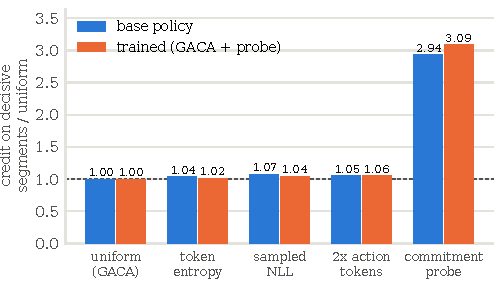
\includegraphics[width=\linewidth]{figs/oracle.pdf}
\caption{\textbf{Credit on decisive segments relative to uniform credit}, by weighting scheme, on held-out
games, for the base policy and for the final policy of the COMMIT training run. Unclipped
segment weights; the clipped training configuration gives $1.65\times$ and $1.64\times$.}
\label{fig:oracle}
\end{figure}

\paragraph{Robustness at the training configuration.}
\Cref{fig:robust} evaluates the exact function used in training (clip $[0.25, 4]$, mean-preserving). It
gives $1.65\times$ (CI $[1.57, 1.74]$) and beats uniform on 80\% of steps. The effect holds for every
task type ($1.52$ to $1.96\times$), for both halves of the games (1.73 and 1.57), for early and late steps,
and with cuts up to three times coarser (1.53). It is largest where it matters most, on steps whose
decision was open ($2.37\times$ against $1.33\times$ when settled). The clip trades concentration for
stability: unclipped weights give $2.18\times$, a $[0.5, 2]$ clip $1.26\times$.

\begin{figure}[t]
\centering
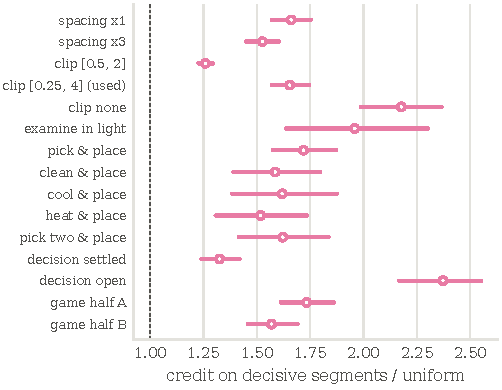
\includegraphics[width=\linewidth]{figs/robust.pdf}
\caption{\textbf{Robustness of probe weights} at the training configuration: credit on decisive
segments relative to uniform with 95\% bootstrap intervals, by cut spacing, clip, task type, decision
openness and game half.}
\label{fig:robust}
\end{figure}

\subsection{Does attention locate it?}
\label{sec:attention}
Bogdan~\etal~\cite{bogdan2025anchors} use attention between sentences as a white-box alternative to
resampling. A transformer computes, for each query token, a softmax-normalized distribution over
earlier keys, $\mathrm{softmax}(QK^\top/\sqrt{d})$~\cite{vaswani2017attention}. We read the attention
that the command tokens pay to each reasoning token, averaged over heads and over the last third of
the layers, and score it like a weighting scheme on 128 held-out steps, restricted to the reasoning
segments (where attention is defined) and compared with the probe on the same segments. Attention does
point toward the decision, but weakly: it places $1.12\times$ more credit on decisive segments than
uniform (CI $[1.03, 1.24]$), against $1.61\times$ ($[1.45, 1.77]$) for the probe on the same steps, and
its per-step rank correlation with importance density is only 0.14. \Cref{fig:example} shows why on
one step. More than half of the decision is settled in the single segment ``\emph{[let's check] the
drawers to see if any have}'', which commits the agent to searching the drawers before it writes
\texttt{go to drawer 1}. The probe puts its weight there. Attention is diffuse and peaks on the
tokens just before the action tag, which is consistent with the view that attention weights are not, by
themselves, explanations~\cite{jain2019attention}.

\begin{figure*}[t]
\centering
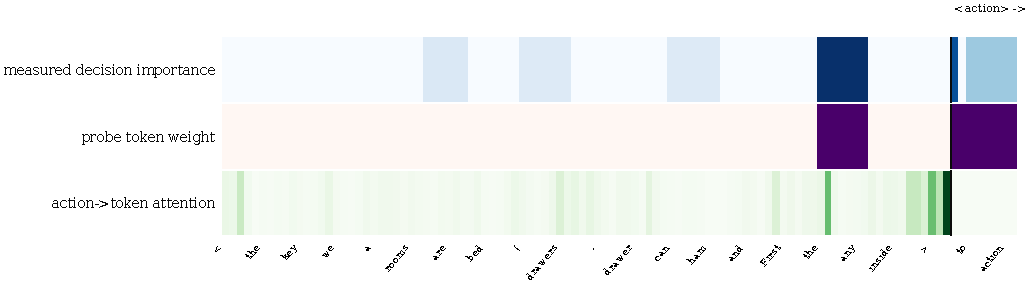
\includegraphics[width=\linewidth]{figs/example.pdf}
\caption{\textbf{One held-out step, token by token.} Top: decision importance measured by the flip
test (darker = more of the decision settled there). Middle: COMMIT credit. Bottom: attention
from the command tokens to each reasoning token (last third of the layers, mean over heads). The
vertical line marks the \texttt{<action>} tag. The task is to put a keychain on a desk; before any
reasoning the eventual command has probability $q(0) = 0.04$ and resampling the whole response changes
it 75\% of the time. 53\% of the decision is settled in one segment, ``the drawers to see if any
have'', where the probe also concentrates its weight; attention is spread out and peaks next to the
action tag.}
\label{fig:example}
\end{figure*}

\subsection{The probe survives training}
The flip test above uses the base policy. Repeating it on the same held-out games with the final weights
of our COMMIT training run gives the same picture: the probe's credit on decisive segments is
$1.64\times$ at the training configuration (CI $[1.55, 1.72]$; base model $1.65\times$) and $3.09\times$
unclipped, entropy stays near $1\times$, and the share of the decision inside the action tags moves only
from 18\% to 21\%. Training does not degrade the probe as a measurement of where decisions are made.
